\begin{figure*}[t]
\begin{tabular}{c c}
	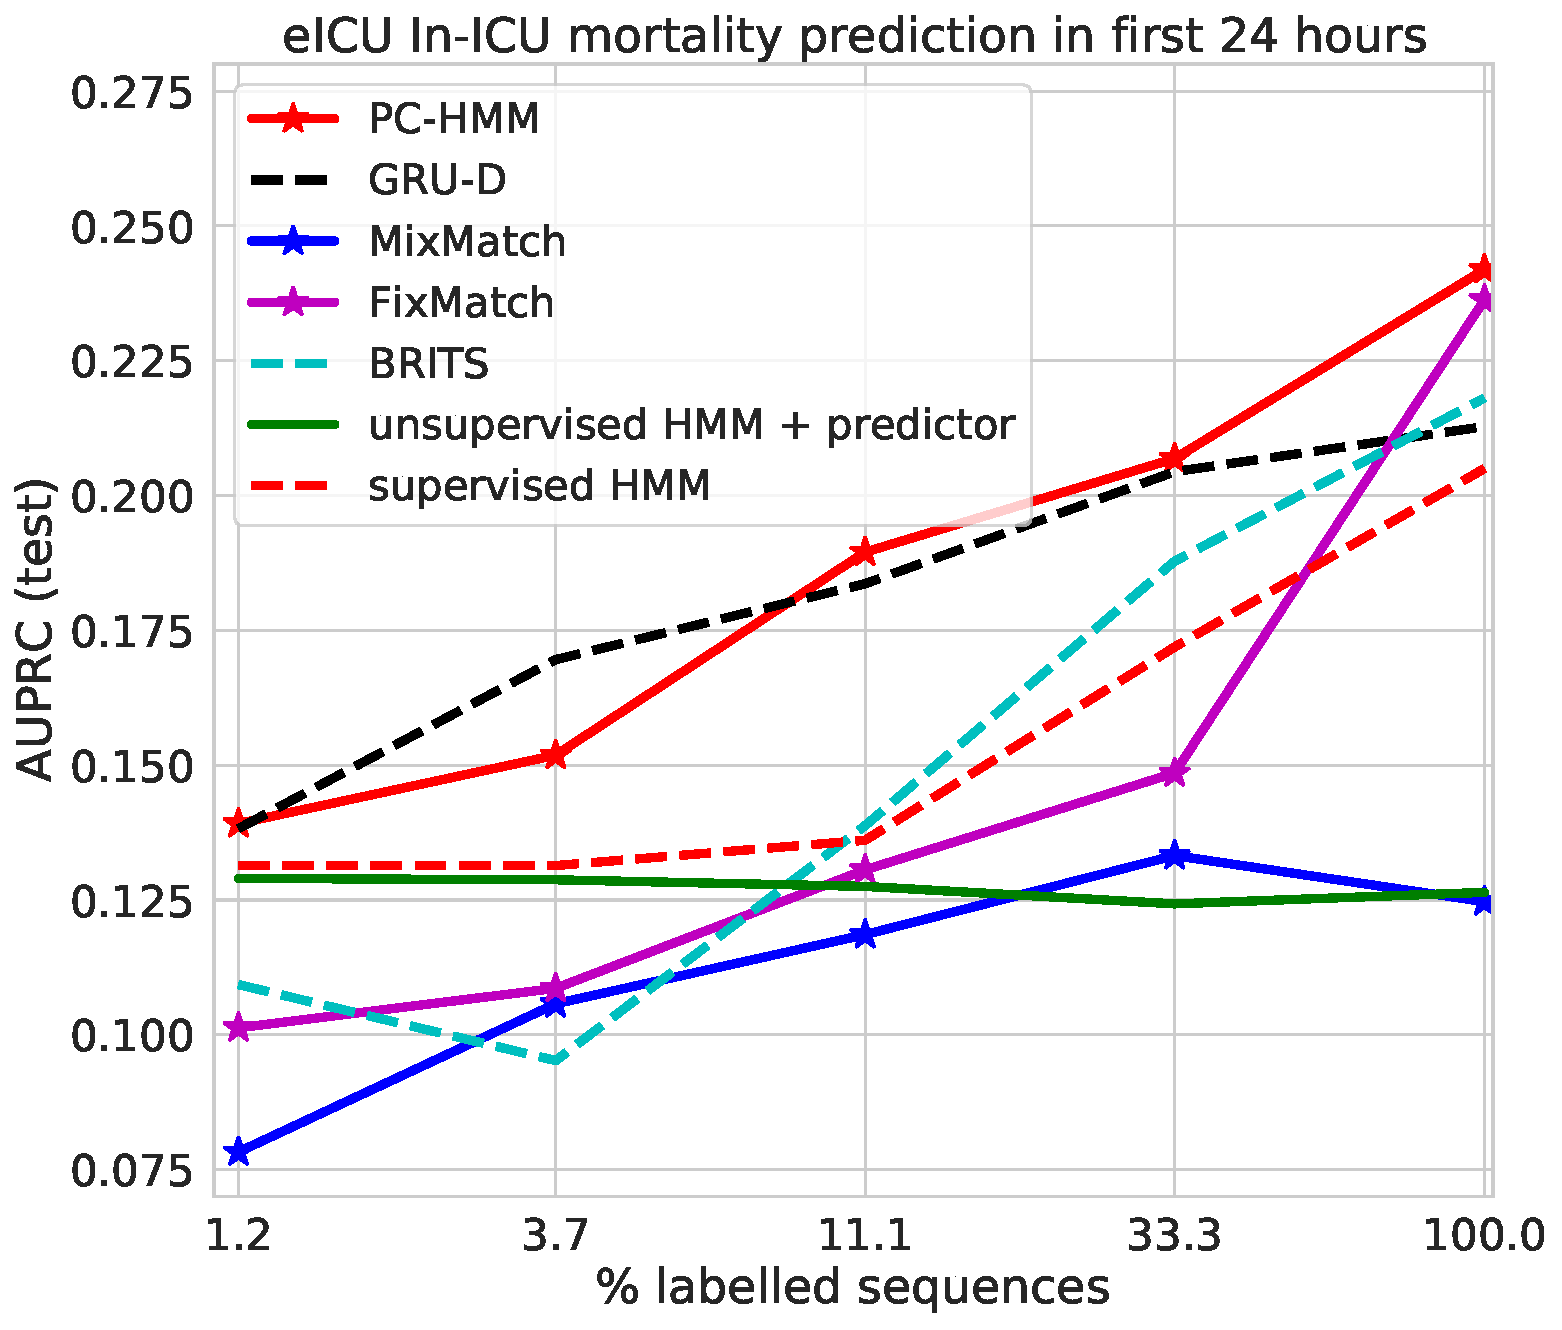
\includegraphics[width=0.5\textwidth]{content/chapters/semi_supervised_pchmm_missing_data/images/perf_mortality_prediction_eicu.pdf}
	&
	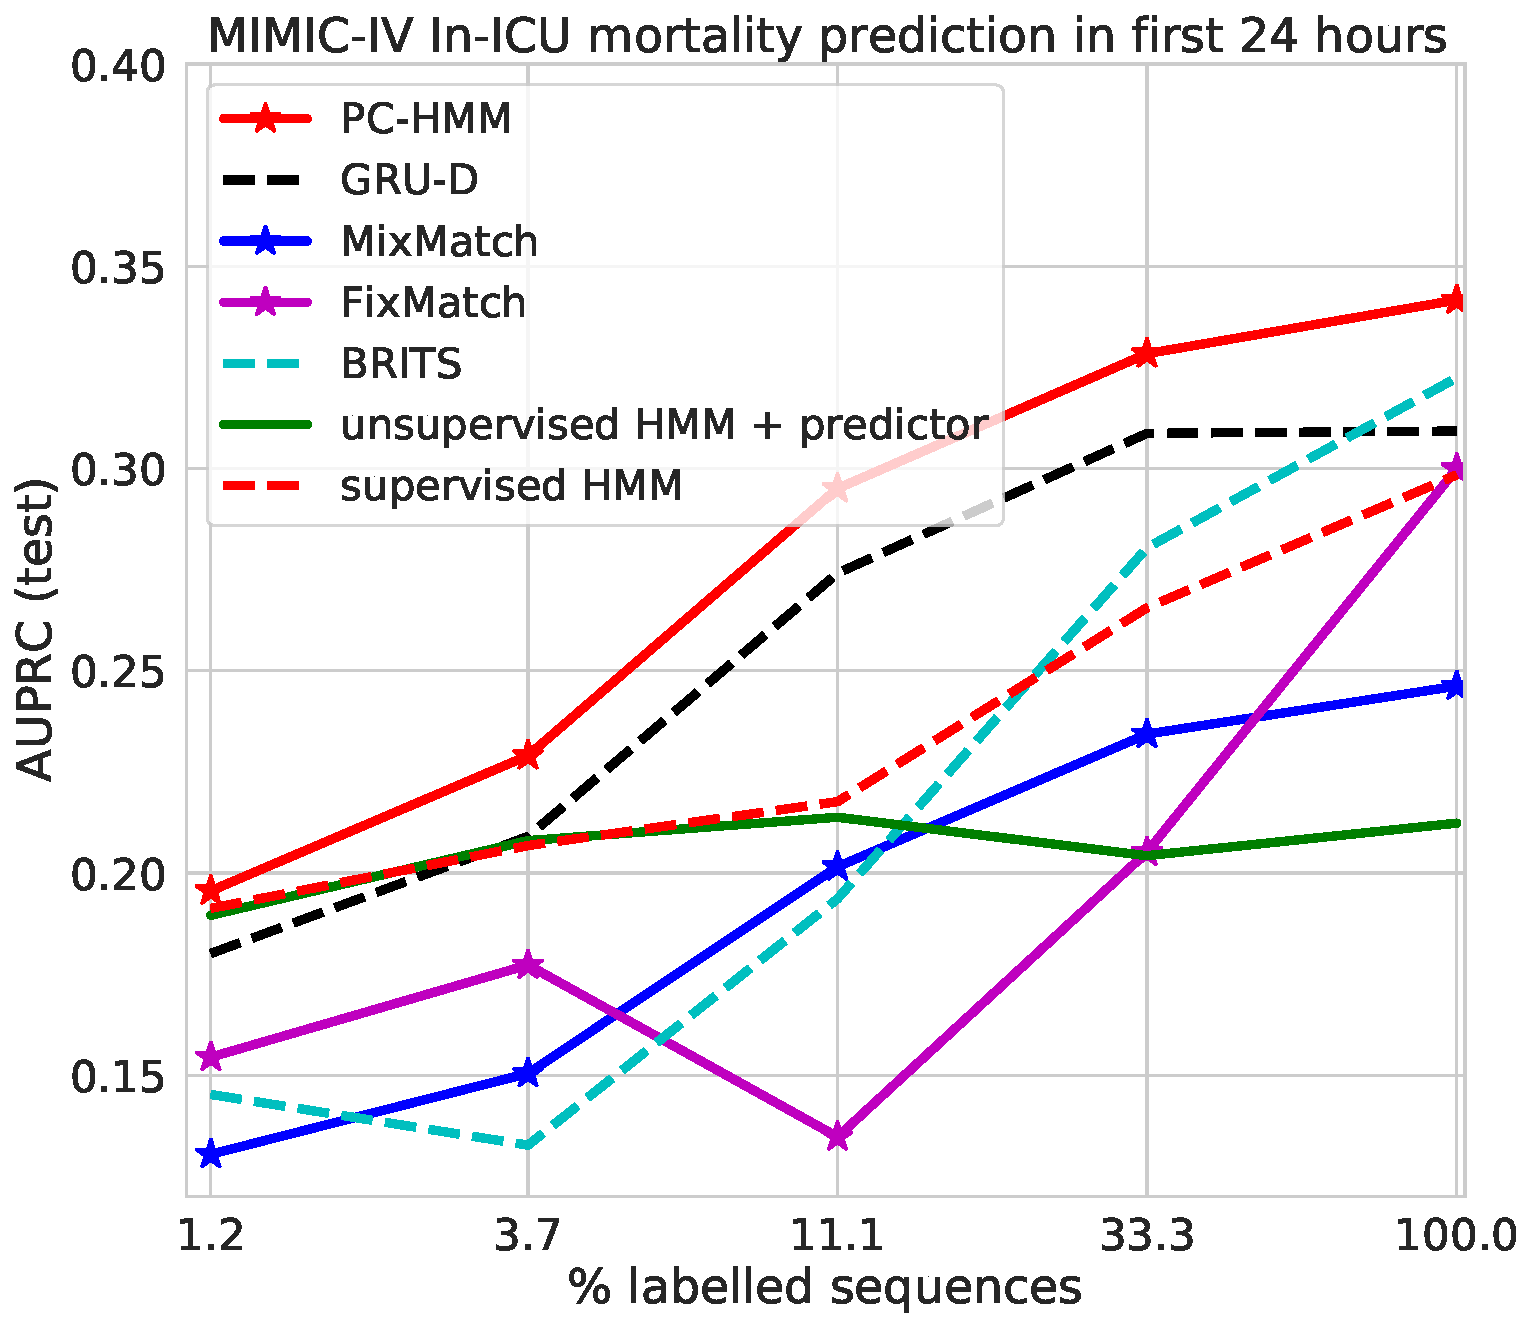
\includegraphics[width=0.5\textwidth]{content/chapters/semi_supervised_pchmm_missing_data/images/perf_mortality_prediction_mimic.pdf}	
\end{tabular}
\caption[AUPRC versus amount of labeled data for in-hospital
mortality early warning classifiers on two large EHR datasets]{AUPRC (higher is better) versus amount of labeled data for in-hospital mortality early warning classifiers on two large EHR datasets (left: eICU, right: MIMIC-IV).
X-axis: Percentage of all training sequences available with labels (SSL methods treat remaining sequences as unlabeled; other methods discard them).
Y-axis: Area under precision-recall curve (AUPRC, higher is better).
%Each line represents a different model.
SSL methods, including our PC-HMM as well as MixMatch and FixMatch,
learn from both labeled and unlabeled data.
GRU-D, BRITS, and Random Forest use the labeled set only.
The PC-HMM matches or beats the other models across all tested labeled set sizes, despite needing fewer parameters and only $1/10^{th}$ of the training time as the other models. }%endcaption

\label{fig:mortality_prediction_results}
\end{figure*}